\documentclass[../ai_in_finance]{subfiles}
\usepackage[margin=1in]{geometry}
\usepackage{tikz}
\usetikzlibrary{positioning}
\usepackage{amsmath}
\usepackage{amssymb}
\usepackage{booktabs}
\usepackage{draftwatermark}

\SetWatermarkText{Wulin.Suo@Queensu.ca}
\SetWatermarkScale{1.4}
\SetWatermarkColor{gray!35}
\SetWatermarkAngle{45}

\usepackage{makeidx}
\makeindex

\begin{document}

\chapter{Explainability, Fairness, and Regulation}

\section{Introduction}

Every applied chapter so far has, at some point, flagged the same unresolved obligation and deferred it here. Chapter 1 warned that a model too opaque to explain to a risk committee is often not deployable at all, whatever its statistical performance. Chapter 5 showed that collapsing two defensible valuations into one confident-looking number can hide a genuine, economically meaningful disagreement, and named preserving that kind of interpretability as a theme the book would return to directly. Chapter 6 noted that regulation constrains how opaque a credit or insurance model can be, and that the importance of interpretability is itself one of the criteria for choosing among competing algorithms. Chapter 13 observed that a suspicious activity report or an account closure decision frequently must be explained to a regulator or a customer, limiting how much a fraud or anti-money-laundering program can lean on its least interpretable models. Chapter 14 made the same point about a trading decision or disclosure classification driven by an attention-based language model. Chapter 15 showed that a convolutional or recurrent network's learned filters and hidden states are far less directly inspectable than a single regression coefficient, a tension that only sharpens as a model's input becomes something as opaque to manual review as a stack of satellite pixels. This chapter is where all of these deferred obligations are finally paid off, not as an afterthought bolted onto a finished model, but as a technical and regulatory discipline with its own methods, worked examples, and open problems.

The chapter is organized around three questions a financial institution must answer before, during, and after deploying a model, mirrored in its three planned subsections: what can be said about \emph{why} a model produced a given output (interpretable and explainable AI), whether the model treats people and groups \emph{fairly} under one or more competing legal and ethical definitions of fairness (ethical and regulatory considerations), and whether the model keeps working as intended once it is deployed, monitored, and eventually attacked or gamed (robustness, governance, and responsible AI). Twelve worked examples run throughout, each reusing a model or dataset from an earlier chapter rather than inventing an isolated one, because explainability and fairness are properties of a model's actual behavior on real cases, not abstract add-ons: permutation feature importance and partial dependence on Chapter 13's fraud-scoring logistic regression\index{logistic regression}, an exact Shapley-value decomposition and a counterfactual explanation\index{counterfactual explanation} for Chapter 9's declined loan applicant, a locally interpretable surrogate model built around Chapter 6's toy feedforward network, a two-group fairness audit and adverse-action reason codes built on the same credit-scoring model, an adversarial ``structuring'' perturbation against the fraud model that extends Chapter 13's money-laundering vocabulary to model evasion directly, and a population stability index\index{population stability index (PSI)} quantifying score drift as a complement to Chapter 13's precision-drift monitoring, and, going a level deeper still, a cost-weighted algorithmic-recourse comparison and an integrated-gradients attribution that revisits Chapter 6's network a second time to show exactly where a naive local-gradient shortcut fails and a proper path integral does not. A real-world case vignette, the 2019 Apple Card\index{Apple Card gender-bias controversy} gender-bias controversy and its regulatory aftermath, ties the chapter's methods back to a dispute that was, at its core, exactly the kind of explainability and fairness question this chapter formalizes, and a second vignette on Upstart Network\index{Upstart Network}'s regulatory engagement with the CFPB shows the same underlying concerns handled proactively rather than after the fact.

\section{Why Financial AI Needs a Theory of Explanation}\index{Why Financial AI Needs a Theory of Explanation}
\label{sec:xai-why}

Suppose a bank's model validation team asks a data scientist why the credit model just denied a particular applicant, and the honest answer is ``because that is what several hundred decision trees, averaged together, produced.'' That answer is true, but it satisfies no one: not the applicant, who is legally entitled under fair-lending rules to specific reasons for the denial; not the regulator, who needs some way to verify the model is not proxying for a protected characteristic; and not the risk committee, who cannot sign off on a decision it cannot itself understand. Two related but distinct words recur throughout this chapter in response to exactly this problem, and are worth fixing precisely before using them interchangeably, as casual usage often does. \textbf{Interpretability} is a property of a model itself: a model is interpretable to the degree that a human can understand, without any additional tool, how its inputs map to its outputs, simply by inspecting its structure. A linear regression's coefficients, Chapter 6's credit-spread regression among them, are interpretable in this direct sense: the coefficient itself is the answer to ``how much does the prediction change per unit change in this feature.'' \textbf{Explainability}, by contrast, is a property of a method applied \emph{after} a model is built, regardless of the model's own structure: an explanation method takes a model, interpretable or not, and produces a human-comprehensible account of a specific prediction or of the model's behavior in general. A deep neural network is not interpretable in the first sense, its millions of weights admit no direct reading, but it can still be explained, approximately, using the post-hoc methods this chapter develops. Every explanation method in this chapter falls into one of four cells formed by two independent distinctions, illustrated in Figure~\ref{fig:xai_taxonomy}: whether it explains the model's behavior in general (\emph{global}) or a single prediction (\emph{local}), and whether it is built into the model's own structure (\emph{intrinsic}) or applied afterward to an already-fit model (\emph{post-hoc}).

\begin{figure}[htbp]
    \centering
    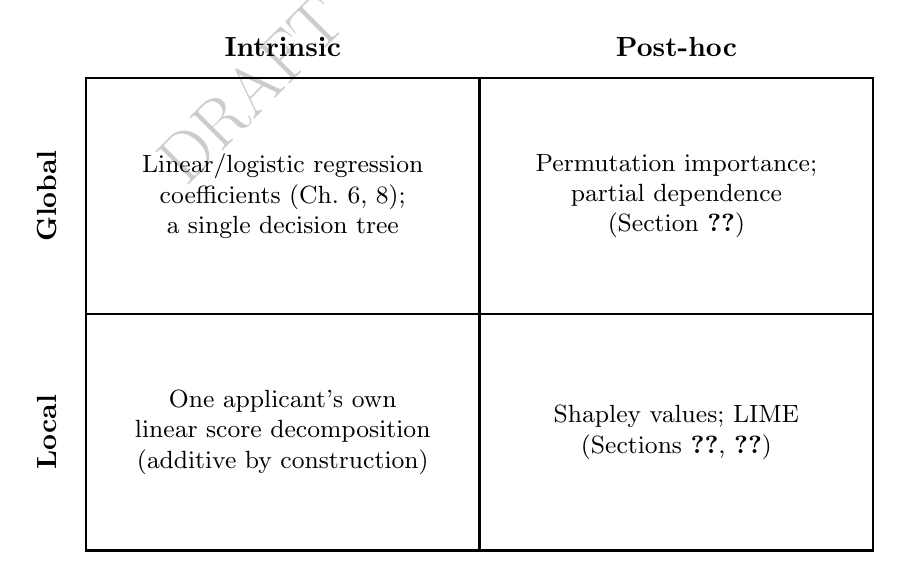
\begin{tikzpicture}[>=latex,thick]
        \draw[thick] (0,0) rectangle (10,6);
        \draw[thick] (5,0) -- (5,6);
        \draw[thick] (0,3) -- (10,3);
        \node at (2.5,6.4) {\textbf{Intrinsic}};
        \node at (7.5,6.4) {\textbf{Post-hoc}};
        \node[rotate=90] at (-0.5,4.5) {\textbf{Global}};
        \node[rotate=90] at (-0.5,1.5) {\textbf{Local}};
        \node[align=center,font=\small] at (2.5,4.5) {Linear/logistic regression\\coefficients (Ch.~6, 8);\\a single decision tree};
        \node[align=center,font=\small] at (7.5,4.5) {Permutation importance;\\partial dependence\\(Section~\ref{sec:global-explain})};
        \node[align=center,font=\small] at (2.5,1.5) {One applicant's own\\linear score decomposition\\(additive by construction)};
        \node[align=center,font=\small] at (7.5,1.5) {Shapley value\index{Shapley value}s; LIME\index{LIME (Local Interpretable Model-agnostic Explanations)}\\(Sections~\ref{sec:shapley-explain}, \ref{sec:lime-explain})};
    \end{tikzpicture}
    \caption{A taxonomy of explanation methods along two axes: global versus local, and intrinsic versus post-hoc. Most of the powerful, high-capacity models this book has introduced, ensembles (Chapter 6), CNNs and RNNs (Chapter 15), transformers (\index{transformer architecture}Chapter 14), fall outside the left column entirely, which is exactly why the post-hoc methods on the right exist.}
    \label{fig:xai_taxonomy}
\end{figure}

The trade-off this taxonomy makes visible is not a minor implementation detail; it is the central tension of this entire chapter. Chapter 6 already observed that the most flexible, highest-capacity models, large ensembles, deep neural networks, are typically also the least directly interpretable, while the most interpretable models, a linear regression, a shallow decision tree, are typically less flexible and can fit a smaller class of relationships. Post-hoc explanation methods do not eliminate this trade-off; they manage it, by producing an approximate, human-readable account of a black-box model's behavior without changing the underlying model at all. That approximation is genuinely useful, a bank can keep the gradient-boosted model that best predicts default while still producing an adverse-action notice for a declined applicant, but it is an approximation, and Section~\ref{sec:lime-explain}'s worked example shows concretely both how well such an approximation can work near the point it is built around and how it can degrade away from that point.

\section{Intrinsically Interpretable Models Revisited}\index{Intrinsically Interpretable Models Revisited}
\label{sec:intrinsic-models}

Before turning to the post-hoc methods that occupy the rest of this chapter, it is worth taking seriously the option of simply choosing a model that needs no post-hoc explanation at all, the left column of Figure~\ref{fig:xai_taxonomy}. Chapter 6 already introduced the two workhorses of this column: linear and logistic regression, whose coefficients are themselves the explanation, and a single decision tree, whose sequence of if-then splits can be read directly as a chain of human-comprehensible rules (``if debt-to-income exceeds 30\% and credit history is under two years, predict default''). Chapter 9's credit-scoring model and Chapter 13's fraud-scoring model, both logistic regressions, were deliberately built this way, and Section~\ref{sec:shapley-explain}'s exact, closed-form Shapley decomposition was only possible because of it; a bank that can accept a small accuracy cost in exchange for this kind of direct interpretability avoids the entire post-hoc apparatus this chapter otherwise requires.

Two refinements extend this intrinsic column considerably further than a single linear model or a single tree, without leaving it. A \textbf{generalized additive model (GAM)}\index{Generalized Additive Model (GAM)} replaces logistic regression's linear combination $\beta_0 + \sum_j \beta_j x_j$ with a sum of flexible, individually plotted functions, $\beta_0 + \sum_j f_j(x_j)$, letting each feature's relationship to the outcome be nonlinear (a U-shaped effect of age on default risk, say, rather than a single coefficient forcing a straight line) while keeping the model additive across features, so that each $f_j$ can still be inspected and explained on its own, in exactly the same global, intrinsic sense as a linear coefficient. A \textbf{credit scorecard}\index{Credit Scorecard}, the industry-standard format underlying Chapter 9's $850$-to-$300$ score transformation, takes a related approach in the opposite direction: it bins each feature into a small number of ranges (debt-to-income under 20\%, 20-30\%, over 30\%, for instance), assigns each bin a small integer number of points from a table, and sums the points across features to produce the final score, a format that a loan officer, an auditor, or a regulator can verify by hand, addition and table lookups only, with no matrix algebra or floating-point evaluation at all. Both formats trade away some of a fully flexible model's predictive power, exactly the trade-off Section~\ref{sec:xai-why} named directly, in exchange for landing entirely in the intrinsic column and needing none of Sections~\ref{sec:global-explain} through~\ref{sec:lime-explain}'s machinery, which is precisely why scorecards remain the dominant format for consumer credit underwriting in practice even though tree ensembles and neural networks routinely outperform them on held-out accuracy alone.

\section{Global Explanations: Permutation Importance and Partial Dependence}\index{Global Explanations: Permutation Importance and Partial Dependence}
\label{sec:global-explain}

Suppose a risk manager wants a one-sentence answer to which of the fraud model's three features it actually relies on, before deciding whether it is safe to keep purchasing all three data feeds going forward, without asking a data scientist to walk through a single coefficient. A global explanation answers exactly this by describing a model's behavior across its entire input space, or at least across a representative dataset, rather than for one specific case. \textbf{Permutation feature importance} asks a direct empirical question: how much does the model's performance degrade if a single feature's values are shuffled (permuted) across the dataset, breaking whatever real relationship that feature had with the outcome while leaving every other feature, and the true labels, untouched? A feature whose permutation causes a large performance drop is one the model relies on heavily; a feature whose permutation changes nothing is one the model could apparently do without, at least on this data.

Recall Chapter 13's fraud-scoring logistic regression, fit to ten transactions with three features (amount $z$-score, distance from home in hundreds of kilometers, and a late-night indicator) and coefficients $\hat\beta_0 \approx -2.57$, $\hat\beta_1 \approx 0.83$, $\hat\beta_2 \approx 0.15$, $\hat\beta_3 \approx 0.82$, achieving 90\% accuracy and an $F_1$ of $0.857$ at its 0.5 threshold. Permuting a feature means reassigning its ten values to the ten transactions in a different order; the clearest way to do this by hand is simply to reverse the column, so that transaction 1 receives transaction 10's value for that feature, transaction 2 receives transaction 9's value, and so on, while every other feature and every actual-fraud label stays exactly where it was. Table~\ref{tab:permutation_importance} reports the resulting accuracy and $F_1$ for each of the three features permuted this way, one at a time.

\begin{table}[htbp]
\centering
\caption{Permutation feature importance for the fraud-scoring model}
\label{tab:permutation_importance}
\begin{tabular}{lrrr}
\toprule
Feature permuted & Accuracy & Precision & $F_1$ \\
\midrule
(baseline, no permutation) & 0.900 & 1.000 & 0.857 \\
Amount $z$-score & 0.300 & 0.000 & undefined \\
Distance from home & 0.900 & 1.000 & 0.857 \\
Late-night indicator & 0.900 & 1.000 & 0.857 \\
\bottomrule
\end{tabular}
\end{table}

Reversing the amount $z$-score column is catastrophic: accuracy collapses from 90\% to 30\%, and the model's three flagged transactions after permutation (5, 8, and 10) are all false positives, none of the four genuine frauds is caught, so precision and recall both fall to zero and $F_1$ is undefined (conventionally reported as zero). Reversing either the distance column or the late-night column alone, by contrast, changes not a single one of the ten predictions: accuracy and $F_1$ are identical to the unpermuted baseline. The conclusion is not that distance and late-night timing are irrelevant to fraud in general, Chapter 13's own coefficients show both raise predicted fraud probability, but that for this specific ten-transaction sample, the amount $z$-score so dominates the linear combination that no rearrangement of the other two features' values happens to push any transaction across the 0.5 threshold in either direction. This is exactly the caveat permutation importance always carries: it measures a feature's contribution to performance \emph{on the data at hand}, not some feature's context-free importance, and a feature that appears unimportant here could easily prove decisive on a different, larger sample where its values interact more consequentially with the others.

A complementary global tool, \textbf{partial dependence}, asks a different question: holding the joint distribution of every other feature fixed at its empirical values, how does the model's average prediction change as one feature of interest is swept across a range of values? Formally, the partial dependence of the fraud model on the amount $z$-score $z$ is $\text{PD}(z) = \frac{1}{n}\sum_{i=1}^n \sigma\big(\hat\beta_0 + \hat\beta_1 z + \hat\beta_2 d_i + \hat\beta_3 n_i\big)$, averaging over the ten transactions' actual distance and late-night values while only $z$ is varied. Table~\ref{tab:partial_dependence} evaluates this at six values of $z$.

\begin{table}[htbp]
\centering
\caption{Partial dependence of predicted fraud probability on amount $z$-score}
\label{tab:partial_dependence}
\begin{tabular}{lrrrrrr}
\toprule
Amount $z$-score & $-1$ & 0 & 1 & 2 & 3 & 4 \\
Average predicted probability & 0.095 & 0.185 & 0.320 & 0.489 & 0.663 & 0.807 \\
\bottomrule
\end{tabular}
\end{table}

The curve crosses the 0.5 classification threshold between $z=2$ and $z=3$, at approximately $z \approx 2.07$, meaning that an otherwise-typical transaction (average distance and late-night status across the sample) is predicted fraudulent once its amount is roughly two standard deviations above the cardholder's usual spending. Partial dependence and permutation importance answer different questions and can disagree: a feature can have a smooth, informative partial-dependence curve while still showing zero permutation importance on a specific sample, exactly as distance did above, since partial dependence describes the model's functional form directly while permutation importance describes how much a specific dataset's performance metric happens to depend on that feature.

\section{Local Explanations: Shapley Values for a Single Decision}\index{Local Explanations: Shapley Values for a Single Decision}
\label{sec:shapley-explain}

A global explanation tells a modeler or regulator how a model behaves in general; it does not answer the question an individual declined applicant actually asks, which is why \emph{my} application was denied. A \textbf{Shapley value}, borrowed from cooperative game theory (Shapley, 1953) and popularized in machine learning as SHAP\index{SHAP} (SHapley Additive exPlanations), answers exactly this question by fairly dividing credit for a single prediction's deviation from some baseline among the features that produced it. For a model that is linear in its inputs, exactly the case for Chapter 9's credit-scoring logistic regression's log-odds, the Shapley value has a particularly clean closed form: the contribution of feature $j$ is simply $\hat\beta_j (x_j - \bar x_j)$, the feature's coefficient times its deviation from a reference baseline, and these contributions sum \emph{exactly} to the difference between the individual's predicted log-odds and the baseline's, a property called efficiency that any valid additive attribution must satisfy.

Recall Chapter 9's credit-scoring model,
$$z = -12.152 + 0.530\,(\text{Debt/Income}) - 0.231\,(\text{Credit History})$$ 
(coefficients shown rounded; the fitted model itself carries full floating-point precision), applied to an applicant with a 28\% debt-to-income ratio and 4 years of credit history. To decompose this prediction, a baseline is needed: a natural, already-established choice is the mean applicant in Chapter 6's six-applicant reference population (debt-to-income $\bar x_1 = 26.33\%$, credit history $\bar x_2 = 5.17$ years). Comparing the two,
\begin{align*}
\text{Applicant:} &\quad z \approx 1.761, \ \Pr(\text{Default}) \approx 85.3\%, \ \text{score} \approx 381, \\
\text{Baseline:} &\quad z_{\text{baseline}} \approx 0.608, \ \Pr(\text{Default})_{\text{baseline}} \approx 64.7\%, \ \text{score} \approx 494,
\end{align*}
the applicant's score comfortably below most lenders' approval cutoffs, the baseline itself a subprime score but far less severe.

The Shapley decomposition of the gap between them is
\begin{equation*}
\underbrace{1.761}_{z_{\text{applicant}}} = \underbrace{0.608}_{z_{\text{baseline}}} + \underbrace{0.530\,(28 - 26.33)}_{\text{debt-to-income contribution} \,=\, 0.883} + \underbrace{(-0.231)\,(4 - 5.17)}_{\text{credit-history contribution} \,=\, 0.270},
\end{equation*}
and indeed $0.608 + 0.883 + 0.270 = 1.761$ exactly, up to rounding, verifying the efficiency property directly. Both features push the applicant's predicted risk above the baseline, the applicant's debt-to-income ratio is higher than the reference population's average (more leverage, more risk) and the applicant's credit history is shorter than average (less seasoning, more risk), but debt-to-income's contribution (0.883) is more than three times credit history's (0.270), identifying debt-to-income as the dominant driver of this applicant's elevated predicted default risk, not merely a contributing factor tied for first place. Figure~\ref{fig:shap_waterfall} draws this decomposition as a waterfall chart, the standard way a SHAP explanation is presented in practice.

\begin{figure}[htbp]
    \centering
    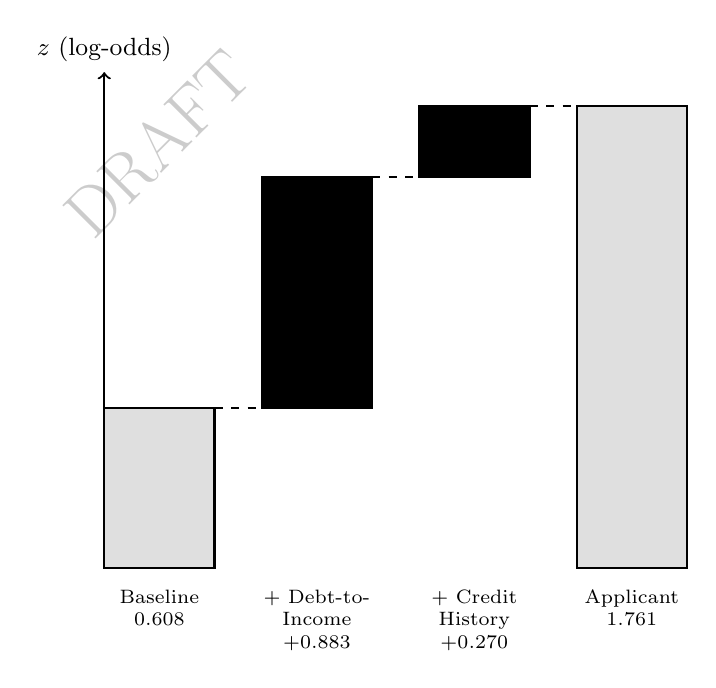
\begin{tikzpicture}[thick]
        \draw[->] (0,0) -- (0,6.3) node[above,font=\small] {$z$ (log-odds)};
        \draw[fill=gray!25] (0,0) rectangle (1.4,2.03);
        \node[below,font=\scriptsize,align=center] at (0.7,-0.15) {Baseline\\$0.608$};
        \draw[fill=black] (2,2.03) rectangle (3.4,4.97);
        \node[below,font=\scriptsize,align=center] at (2.7,-0.15) {$+$ Debt-to-\\Income\\$+0.883$};
        \draw[fill=black] (4,4.97) rectangle (5.4,5.87);
        \node[below,font=\scriptsize,align=center] at (4.7,-0.15) {$+$ Credit\\History\\$+0.270$};
        \draw[fill=gray!25] (6,0) rectangle (7.4,5.87);
        \node[below,font=\scriptsize,align=center] at (6.7,-0.15) {Applicant\\$1.761$};
        \draw[dashed] (1.4,2.03) -- (2,2.03);
        \draw[dashed] (3.4,4.97) -- (4,4.97);
        \draw[dashed] (5.4,5.87) -- (6,5.87);
    \end{tikzpicture}
    \caption{The Shapley decomposition as a waterfall chart. Starting from the baseline applicant's log-odds ($0.608$), each feature's contribution (black bars) bridges the gap to the actual applicant's log-odds ($1.761$, right), with debt-to-income responsible for more than three times the credit-history contribution.}
    \label{fig:shap_waterfall}
\end{figure}

\subsection*{From Shapley Values to Adverse Action Reason Codes}\index{From Shapley Values to Adverse Action Reason Codes}
\label{sec:adverse-action}

This decomposition is not merely an academic exercise: it is, in substance, exactly what U.S. law already requires a lender to produce. The Equal Credit Opportunity Act\index{Equal Credit Opportunity Act (ECOA)} and its implementing Regulation B\index{Regulation B} require that a lender who denies credit furnish the applicant with the specific, principal reasons for the denial, an \emph{adverse action notice}, rather than a bare rejection. Ranking the Shapley contributions above by magnitude produces precisely this: ``high debt-to-income ratio relative to similar applicants'' as the principal reason (contribution 0.883), and ``limited length of credit history'' as a secondary, contributing reason (contribution 0.270). This works cleanly here because the underlying model is linear in the log-odds, so the Shapley value has an exact closed form; for a nonlinear model such as a gradient-boosted ensemble, the same additive decomposition can still be computed, using the general (and considerably more expensive) Shapley formula that averages a feature's marginal contribution over every possible ordering of the other features, which is precisely why fast approximations to full Shapley computation, and simpler surrogate methods like Section~\ref{sec:lime-explain}'s, remain an active area of applied research.

\subsection*{Counterfactual Explanations: How Much Would Need to Change?}\index{Counterfactual Explanations: How Much Would Need to Change}
\label{sec:counterfactual}

A closely related, and often more actionable, form of explanation answers a different question: not why was I denied, but what is the smallest change that would have gotten me approved? Suppose this lender approves any applicant with a credit score of at least 620, equivalent to 
$$\Pr(\text{Default}) \le \frac{850-620}{550} \approx 41.8\%,$$ 
or $z \le -0.330$. Holding the applicant's 4 years of credit history fixed and solving 
$$-12.152 + 0.530\,(\text{DTI}) - 0.231(4) = -0.330$$ 
for debt-to-income gives $\text{DTI} \approx 24.05\%$, a reduction of about 3.95 percentage points from the applicant's actual 28\%. This \emph{counterfactual explanation}, reduce your debt-to-income ratio by roughly four percentage points, holding everything else fixed, and this same model would approve you, is often more useful to a declined applicant than a bare coefficient or a Shapley value, since it states a concrete, achievable target rather than merely a ranked list of contributing factors, though it shares the same important caveat as Section~\ref{sec:lime-explain}'s local surrogate: it describes what would happen if only debt-to-income changed and nothing else about the applicant's profile shifted along with it, an assumption that is convenient for exposition but not guaranteed to hold in reality.

\section{Local Surrogate Models: LIME for a Genuinely Nonlinear Model}\index{Local Surrogate Models: LIME for a Genuinely Nonlinear Model}
\label{sec:lime-explain}

Shapley values have an exact closed form for Chapter 9's credit-scoring model only because that model is linear in the log-odds; most of the flexible models this book has introduced, Chapter 6's ensembles, Chapter 15's CNNs and RNNs, are not. \textbf{LIME} (Local Interpretable Model-agnostic Explanations) handles this case differently: rather than working out an exact decomposition analytically, it treats the model as a black box, samples a handful of points in the neighborhood of the specific input to be explained, records the black box's predictions at each sampled point, and fits a simple, interpretable model, ordinarily a weighted linear regression, to those sampled input-output pairs. The fitted local model's coefficients are then reported as the explanation, valid, by construction, only in the neighborhood the samples were drawn from.

Recall Chapter 6's small feedforward network, two inputs, a hidden layer of two ReLU units, and a sigmoid output, with weights 
$$W_1 = \begin{pmatrix}0.4 & -0.2\\ 0.1 & 0.3\end{pmatrix},\ b_1 = \begin{pmatrix}0.05\\-0.1\end{pmatrix},  \ W_2 = \begin{pmatrix}0.6 & -0.5\end{pmatrix}, \ b_2 = 0.1,$$ 
which at $x_0 = (1.0, 0.5)$ produces hidden activations $h_0 = (0.35, 0.15)$ and a prediction $\hat y_0 \approx 0.558$. Because both ReLU units are active (their pre-activations are positive) at $x_0$, the network is, in a small enough neighborhood, exactly linear there, so this example doubles as a check on LIME's method: the fitted local surrogate should recover the true local behavior almost exactly, not merely approximately. Table~\ref{tab:lime_samples} lists eight perturbed points around $x_0$, each within $\pm 0.1$ of $x_0$ in each coordinate, and the network's exact prediction at each.

\begin{table}[htbp]
\centering
\caption{Perturbed samples around $x_0=(1.0,0.5)$ and the network's exact prediction}
\label{tab:lime_samples}
\begin{tabular}{lrr}
\toprule
Perturbed input $(x_1,x_2)$ & Hidden activations & Prediction $\hat y$ \\
\midrule
$(1.1, 0.5)$ & $(0.39, 0.16)$ & 0.5632 \\
$(0.9, 0.5)$ & $(0.31, 0.14)$ & 0.5538 \\
$(1.0, 0.6)$ & $(0.33, 0.18)$ & 0.5518 \\
$(1.0, 0.4)$ & $(0.37, 0.12)$ & 0.5651 \\
$(1.1, 0.6)$ & $(0.37, 0.19)$ & 0.5565 \\
$(0.9, 0.4)$ & $(0.33, 0.11)$ & 0.5605 \\
$(1.1, 0.4)$ & $(0.41, 0.13)$ & 0.5698 \\
$(0.9, 0.6)$ & $(0.29, 0.17)$ & 0.5471 \\
\bottomrule
\end{tabular}
\end{table}

Fitting an ordinary least-squares surrogate 
$$\hat y \approx a + b_1 x_1 + b_2 x_2$$ 
to these eight samples gives $a \approx 0.545$, $b_1 \approx 0.0468$, $b_2 \approx -0.0666$. The analytical local gradient, obtained by differentiating the network directly (valid precisely because both ReLU units stay active throughout this neighborhood), is $\frac{\partial \hat y}{\partial x} = \hat y_0(1-\hat y_0)\, W_2 W_1 \approx (0.0469, -0.0666)$, matching the LIME-fitted slope to three decimal places. Evaluating the fitted surrogate at $x_0$ itself gives $\hat y_{\text{surrogate}}(x_0) \approx 0.558$, matching the network's true output $0.558$ almost exactly, exactly the local-fidelity property LIME is designed to deliver. This agreement is not a coincidence of this particular network; it is a direct consequence of the neighborhood chosen being small enough that no ReLU unit crosses its activation boundary. Perturbing further away breaks this: at $x = (1.0, -0.1)$, the second hidden unit's pre-activation is exactly zero and the ReLU clips it, giving a true prediction of $\hat y \approx 0.594$, while the local surrogate fitted above, extrapolated to this same point, predicts approximately $0.598$, a small but growing discrepancy that would widen further still at points beyond it. LIME's neighborhood radius is therefore not a mathematical given but a modeling choice with real consequences: too narrow, and the explanation is trivially accurate but uninformative about the model's broader behavior; too wide, and it silently averages over a region where the black box's true behavior is no longer linear at all, understating exactly the kind of kinked, nonlinear behavior that motivated using a deep model in the first place.

\section{International Regulatory Approaches to Explainability}\index{International Regulatory Approaches to Explainability}
\label{sec:reg-approaches}

Section~\ref{sec:adverse-action} described the U.S. approach to mandated explanation, the Equal Credit Opportunity Act's adverse-action notice requirement, which is principles-based: it specifies the outcome a lender must produce (specific, principal reasons for a denial) without prescribing which technical method must be used to produce it, which is exactly why Section~\ref{sec:shapley-explain}'s exact Shapley decomposition and a scorecard's summed points from Section~\ref{sec:intrinsic-models} are equally acceptable ways of satisfying it. The European Union's approach is both broader in scope and, in places, more prescriptive. The General Data Protection Regulation (GDPR)\index{General Data Protection Regulation (GDPR)}'s Article 22 grants individuals a right not to be subject to a decision based solely on automated processing that produces legal or similarly significant effects, which credit and insurance underwriting plainly are, and Article 13-15 read alongside it are generally understood to require that the individual be given at least meaningful information about the logic involved, sometimes summarized as a ``right to explanation,'' although the precise technical content this requires (a global description of the model's logic, as most regulators and commentators read it, versus an individualized explanation of the specific decision, a stronger reading some have argued for) remains genuinely contested among legal scholars, a rare case in this book where the technical machinery, Section~\ref{sec:shapley-explain} and \ref{sec:lime-explain}'s methods, is more settled than the legal question of exactly how much of it the law actually demands.

The EU's more recent Artificial Intelligence Act\index{EU Artificial Intelligence Act} goes further still, moving from a data-protection framing to a product-safety one: it classifies creditworthiness assessment and credit-scoring systems explicitly as ``high-risk AI'' (Annex III), a category that triggers concrete, ex-ante obligations before deployment, a documented risk-management system, technical documentation sufficient for a regulator to audit, human oversight capable of overriding the system, and demonstrated accuracy, robustness, and cybersecurity, rather than the U.S. framework's more reactive, per-decision adverse-action obligation. A financial institution operating in both jurisdictions therefore faces two different compliance postures on the same underlying model: the U.S. framework asks it to explain individual outcomes after the fact and to avoid disparate impact in aggregate (Section~\ref{sec:fairness}), while the EU framework asks it to certify the system's design, documentation, and human oversight before the model is ever used to score a single real applicant, a genuine example of the same technical toolkit, Sections~\ref{sec:global-explain} through~\ref{sec:lime-explain}, being pressed into service to satisfy two structurally different regulatory philosophies at once.

\section{Fairness in Financial AI}\index{Fairness in Financial AI}
\label{sec:fairness}

Explainability answers what drove a specific decision; fairness asks a related but logically separate question, whether a model's decisions, however well explained, treat different groups equitably. Financial regulators have historically operationalized this through two, not entirely compatible, statistical definitions, and a substantial body of theoretical work has shown that this incompatibility is not a matter of insufficiently clever engineering but a mathematical impossibility in general.

\textbf{Disparate impact and the four-fifths rule\index{four-fifths rule}.} A lending, hiring, or underwriting practice exhibits disparate impact if it produces substantially different outcome rates across groups, even when no feature encodes group membership directly and no discriminatory intent can be shown. U.S. regulatory guidance operationalizes ``substantially different'' using the \emph{four-fifths rule}: if the group with the lower favorable-outcome rate receives that outcome less than 80\% as often as the group with the higher rate, the \emph{adverse impact ratio\index{adverse impact ratio}}, 
$$\text{AIR} = \frac{\min(\text{rate}_A, \text{rate}_B)}{\max(\text{rate}_A, \text{rate}_B)},$$ 
falls below 0.80, disparate impact is presumed and the practice invites regulatory scrutiny regardless of intent.

\textbf{Equalized odds\index{Equalized Odds} and error-rate parity.} A second family of definitions asks not whether groups receive the favorable outcome at similar rates, but whether the model is equally \emph{accurate} for each group, specifically, whether its false-negative rate (missing an applicant who will actually default, in this chapter's running example) and false-positive rate are similar across groups. A model can satisfy the four-fifths rule while its false-negative rate is dramatically higher for one group than another, or vice versa, and a substantial theoretical literature (Chouldechova, 2017; Kleinberg, Mullainathan, and Raghavan, 2017, developed originally in the context of criminal-justice risk scores but directly applicable here) proves that, except in the special case where the two groups have identical underlying default rates, no model can simultaneously satisfy calibration\index{calibration}, equal false-negative rates, and equal false-positive rates across groups. A regulator or an internal model-risk function must therefore choose, explicitly, which fairness definition a given model is being held to, rather than assuming that satisfying one automatically satisfies the others.

Table~\ref{tab:fairness_audit} makes this tension concrete with a small, stylized fairness audit of Chapter 9's credit-scoring model applied to two hypothetical four-applicant groups, Alpha and Beta, at the same 620-score approval threshold used in Section~\ref{sec:counterfactual} ($\Pr(\text{Default}) \le 41.8\%$).

\begin{table}[htbp]
\centering
\caption{A fairness audit of the credit-scoring model on two synthetic four-applicant groups}
\label{tab:fairness_audit}
\begin{tabular}{lrrrrl}
\toprule
Applicant & Debt/income & Credit history & $\Pr(\text{Default})$ & Decision & Will actually default \\
\midrule
Alpha-1 & 15\% & 9 yrs & 0.2\% & Approve & No \\
Alpha-2 & 22\% & 6 yrs & 13.2\% & Approve & \textbf{Yes} \\
Alpha-3 & 30\% & 3 yrs & 95.5\% & Deny & Yes \\
Alpha-4 & 18\% & 8 yrs & 1.1\% & Approve & No \\
\midrule
Beta-1 & 25\% & 4 yrs & 54.3\% & Deny & No \\
Beta-2 & 33\% & 2 yrs & 99.2\% & Deny & Yes \\
Beta-3 & 20\% & 5 yrs & 6.2\% & Approve & No \\
Beta-4 & 38\% & 1 yr & $>$99.9\% & Deny & Yes \\
\bottomrule
\end{tabular}
\end{table}

Group Alpha's approval rate is $3/4 = 75\%$; Group Beta's is $1/4 = 25\%$, giving an adverse impact ratio of $0.25/0.75 = 0.333$, far below the 0.80 threshold and, on this evidence alone, a clear four-fifths-rule violation calling for further fair-lending investigation. Yet the error-rate picture is not simply the mirror image of this disparity: among Group Alpha's two applicants who will actually default (Alpha-2 and Alpha-3), the model approves one of them (Alpha-2, whose moderate debt-to-income and credit history keep her predicted probability just under the threshold), a false-negative rate of $50\%$; among Group Beta's two future defaulters (Beta-2 and Beta-4), the model correctly denies both, a false-negative rate of $0\%$. The group that is approved far more often (Alpha) is thus also the group whose true risk the model is worse at catching, while the group facing the harsher approval rate (Beta) is, on this small sample, screened perfectly. Neither statistic alone tells the whole story: a regulator focused only on approval-rate parity would flag this model for disadvantaging Beta, while a regulator focused only on error-rate parity would note that Alpha's approved population is quietly carrying more missed risk, and reconciling the two findings, rather than optimizing either one in isolation, is exactly the judgment call the impossibility result above shows cannot be avoided by a purely statistical fix.

The impossibility result cited above names a third statistic, calibration, worth checking directly rather than only invoking by name. Both groups happen to share an identical actual default rate here, $2/4=50\%$ for Alpha and $2/4=50\%$ for Beta, exactly the special case the impossibility theorem carves out as the one setting where all three properties, calibration, equal false-negative rates, and equal false-positive rates, could in principle coexist. Yet a simple calibration-in-the-large check, comparing each group's average \emph{predicted} default probability to its actual default rate, shows the model is not equally calibrated across them even so:
\begin{align*}
\text{Group Alpha predictions:} &\quad 0.19\%,\ 13.26\%,\ 95.50\%,\ 1.14\% \quad (\text{mean } 27.5\%, \text{ actual } 50\%), \\
\text{Group Beta predictions:} &\quad 54.3\%,\ 99.2\%,\ 6.3\%,\ 99.96\% \quad (\text{mean } 64.9\%, \text{ actual } 50\%),
\end{align*}
the model systematically under-predicts risk for Alpha and over-predicts it for Beta, even though both groups' realized outcomes are identical. This is not a violation of the impossibility theorem, which is a statement about idealized population distributions, not a guarantee about any one small finite sample, but it is a concrete illustration of exactly how the tension it describes actually shows up in practice: equal base rates do not, by themselves, force equal calibration, equal error rates, or equal approval rates in a real, finite population, and a fairness audit that checked only the adverse impact ratio, only the error-rate gap, or only calibration would each tell a different, individually incomplete part of this same story.

\subsection*{Individual Fairness: A Third Paradigm}\index{Individual Fairness: A Third Paradigm}

Both fairness definitions above are \emph{group} fairness notions: they compare an aggregate statistic, an approval rate or an error rate, across two or more predefined groups. A third paradigm, \textbf{individual fairness} (Dwork, Hardt, Pitassi, Reingold, and Zemel, 2012), asks a different question entirely: are two individuals who are similar with respect to the task at hand treated similarly by the model, regardless of which group either belongs to? Formally, this requires a task-specific similarity metric, a notion of distance between applicants that captures what ``similar with respect to creditworthiness'' actually means, and a model satisfies individual fairness if it maps similar inputs to similar outputs under that metric. Table~\ref{tab:fairness_audit}'s Alpha-2 and Beta-3 illustrate why this third lens matters: their predicted default probabilities are 13.2\% and 6.2\% respectively, not identical but broadly comparable, despite belonging to different groups and receiving different final decisions (approved and approved, in this case, though a stricter similarity threshold could flag even this small gap as an individual-fairness violation worth investigating). The practical difficulty individual fairness faces is exactly the difficulty this parenthetical hints at: choosing the similarity metric itself requires the same kind of value judgment, which features count as legitimately relevant to creditworthiness and which do not, that group fairness definitions push onto the choice of protected groups and outcome statistics, so individual fairness does not so much resolve the value judgment Section~\ref{sec:fairness}'s impossibility result identifies as relocate it, from ``which group statistic to equalize'' to ``which similarity metric to adopt.''

\section{Case Vignette: The Apple Card Gender-Bias Controversy}\index{Apple Card Gender-Bias Controversy}
\label{sec:apple-card-vignette}

In November 2019, software entrepreneur David Heinemeier Hansson posted publicly that the Apple Card, issued by Goldman Sachs, had granted him a credit limit twenty times higher than his wife's, despite the couple filing joint tax returns and his wife having a longer credit history and a comparable or better credit score. Apple co-founder Steve Wozniak reported a similar disparity with his own spouse. The claims spread rapidly and prompted the New York State Department of Financial Services to open a formal inquiry into whether Goldman Sachs's credit-limit algorithm violated fair-lending law.

The regulator's eventual findings, published in 2021, illustrate the distinction this chapter has drawn throughout with unusual clarity. The investigation did not find evidence that the algorithm used sex or gender as an input, nor evidence of intentional discrimination under the Equal Credit Opportunity Act, the specific claim the initial controversy had focused on. It did, however, find that Goldman Sachs's underwriting process lacked the kind of testing and monitoring this chapter's Section~\ref{sec:fairness} formalizes: the bank could not adequately demonstrate, after the fact, that its model did not produce disparate outcomes correlated with sex, because it had not systematically tested for this in the way a four-fifths-rule audit like Table~\ref{tab:fairness_audit}'s would, and its customer service representatives, when asked to explain a specific credit-limit decision, could offer no principled, model-derived reason of the kind Section~\ref{sec:adverse-action}'s adverse-action reason codes are designed to produce, only that ``the algorithm decided.'' The regulator's ultimate recommendation was not a fine but a call for stronger fairness testing and clearer consumer-facing explanations of algorithmic credit decisions, precisely the two capabilities this chapter has built by hand. The episode is a useful corrective to a common misreading of fair-lending law: the absence of a protected characteristic as a model input, sometimes called ``fairness through unawareness,'' is neither necessary nor sufficient to avoid disparate impact, since facially neutral inputs correlated with a protected characteristic (a joint account structure that reflects gendered patterns in whose name assets are held, for instance) can reproduce the same disparity a cruder model would have produced by using the protected characteristic directly.

\section{Adversarial Robustness in Financial Models}\index{Adversarial Robustness in Financial Models}
\label{sec:adversarial-robustness}

A model's outputs can be manipulated deliberately, not just misunderstood accidentally, and Chapter 13's fraud and money-laundering vocabulary already has a name for exactly this behavior in a different context: \emph{structuring}, deliberately splitting a transaction to fall just under a reporting or detection threshold. The same idea applies directly to evading a fraud-scoring model rather than a currency-reporting requirement. Recall Chapter 13's transaction 1, an amount $z$-score of 3.1, a distance of 800 kilometers from the cardholder's home, and a late-night flag, correctly flagged as fraud with predicted probability $88.3\%$. Holding distance and late-night status fixed and solving $-2.57 + 0.83\,z + 0.15(8.0) + 0.82(1) = 0$ for $z$ gives $z \approx 0.663$: a fraudster who could somehow disguise this same transaction's amount so that it appears only $0.663$ standard deviations above the cardholder's typical spending, for instance by splitting it into several smaller purchases at the same distant, late-night location, would push the model's prediction just under the 0.5 threshold and evade detection entirely.

This is a substantial required change, a reduction of $2.44$ in the amount $z$-score, not a barely perceptible perturbation, precisely because the transaction's distance and timing already carry so much of the model's suspicion that amount alone cannot be adjusted by a small amount to escape it. This is a meaningfully different, and more reassuring, finding than the classic adversarial-example results in image classification, where an imperceptibly small pixel-level perturbation (Goodfellow, Shlens, and Szegedy, 2015) can flip a deep network's prediction entirely; a low-dimensional, linear-in-the-log-odds model with several independently suspicious features built in, like this fraud-scoring model, is considerably harder to game with a change to any single feature than a high-dimensional deep network is, though it remains vulnerable to an adversary who can jointly manipulate several features at once (reducing amount, choosing a nearby location, and transacting during business hours simultaneously), a joint attack this single-feature analysis does not rule out. This is precisely why Chapter 15's discussion of alternative-data vendor black-box processing and Chapter 13's own point about adversarial adaptation both matter here: any model whose scoring logic can be inferred or guessed by the population it scores, whether by a sophisticated fraud ring or simply by market participants learning which alternative-data patterns a fund's model rewards, will eventually see its inputs shift in response, exactly the concept-drift dynamic Chapter 12 introduced for high-frequency trading models and Chapter 13 quantified for fraud-model precision.

Adversarial robustness, an adversary deliberately crafting an input to fool the model, is a distinct concept from the stress testing\index{stress testing} Chapters 8 and 9 introduced for market and credit risk, subjecting a model or portfolio to an extreme but plausible scenario (a severe recession, a market crash) to see how it behaves, even though both ask a version of ``how does this model behave outside the data it was ordinarily trained on.'' Stress testing probes the model's behavior under a shift in the entire population's characteristics, unemployment rising across the board, say, while adversarial robustness probes its behavior under a targeted, deliberate manipulation of one individual case; a model can be robust to one and vulnerable to the other; a fraud-scoring model retrained frequently enough to handle a genuine, economy-wide shift in spending patterns can still be gamed one transaction at a time by a single sophisticated fraudster, exactly as Section~\ref{sec:adversarial-robustness} showed directly, and a stress-tested credit model that behaves sensibly in a simulated recession offers no particular guarantee about the counterfactual-manipulation risk Section~\ref{sec:counterfactual} raised, an applicant who learns the model's threshold and adjusts a self-reported input specifically to cross it, rather than through any genuine change in creditworthiness.

\section{Model Governance and Monitoring in the AI Era}\index{Model Governance and Monitoring in the AI Era}
\label{sec:governance-monitoring}

Chapters 8 and 9 introduced model risk management\index{model risk management}, independent validation and ongoing performance monitoring for market and credit risk models, and Chapter 13 formalized the three-lines-of-defense structure (business unit, independent compliance and risk function, internal audit) for fraud and anti-money-laundering programs. U.S. bank regulators codify this discipline for essentially every model a bank relies on in a single supervisory guidance document, SR 11-7\index{SR 11-7} (Board of Governors of the Federal Reserve System and Office of the Comptroller of the Currency, 2011), which explicitly names conceptual soundness, ongoing monitoring, and outcomes analysis as the three pillars of sound model risk management, exactly the three capabilities, understanding why a model produces a given output, tracking whether it keeps working, and checking its actual outcomes for fairness, this chapter has built tools for directly.

Chapter 13's precision-drift table tracked a fraud model's precision declining from 24.2\% to 17.1\% over six months as fraudsters adapted their behavior, but precision is a \emph{lagging} indicator: computing it requires investigators to eventually confirm which flagged transactions were genuinely fraudulent, a process that itself takes time. The \textbf{population stability index (PSI)} offers a complementary, \emph{leading} indicator that needs no labels at all, only the model's own score outputs, comparing the distribution of scores in a current period against a baseline distribution established at the time the model was validated. Formally, $\text{PSI} = \sum_{i} (c_i - b_i) \ln(c_i / b_i)$, summed over score bins $i$ with baseline proportion $b_i$ and current proportion $c_i$. Table~\ref{tab:psi_monitoring} illustrates this for the fraud-scoring model, comparing its validation-time score distribution across four bins against a later snapshot.

\begin{table}[htbp]
\centering
\caption{Population stability index for the fraud-scoring model's score distribution}
\label{tab:psi_monitoring}
\begin{tabular}{lrrrrr}
\toprule
Score bin & $[0, 0.25)$ & $[0.25, 0.50)$ & $[0.50, 0.75)$ & $[0.75, 1.00]$ & Total PSI \\
\midrule
Baseline proportion & 0.50 & 0.25 & 0.15 & 0.10 & \\
Current proportion & 0.34 & 0.29 & 0.22 & 0.15 & \\
Bin contribution & 0.062 & 0.006 & 0.027 & 0.020 & 0.115 \\
\bottomrule
\end{tabular}
\end{table}

A total PSI of $0.115$ falls into the conventional ``moderate shift, worth investigating'' band used widely in credit-risk monitoring practice (below $0.10$ is treated as no material change; above $0.25$ as a major shift typically requiring retraining or revalidation before the model continues to be used), well before precision itself has moved enough to be conclusively distinguishable from noise. A larger share of transactions now score in the lower bins and a smaller share in the top bin, consistent with the same adaptive evasion Section~\ref{sec:adversarial-robustness} demonstrated directly: as more transactions structure themselves to sit just under the model's threshold, the population of scores shifts downward even before enough investigated cases accumulate to move the precision figure meaningfully. This is exactly the kind of early warning SR 11-7's ongoing-monitoring pillar is meant to produce, and exactly why a mature model governance program tracks both a leading, label-free statistic like PSI and a lagging, outcome-based statistic like precision, rather than either alone.

The National Institute of Standards and Technology's AI Risk Management Framework (NIST AI RMF\index{NIST AI Risk Management Framework} 1.0, 2023) organizes this entire chapter's concerns, explainability, fairness, robustness, and governance, into a single voluntary framework built around four functions: \emph{govern} (establishing accountability and policy, this chapter's Section~\ref{sec:governance-monitoring} and Chapter 13's three lines of defense\index{three lines of defense}), \emph{map} (understanding a model's context and likely impact, including on different demographic groups, Section~\ref{sec:fairness}), \emph{measure} (the technical methods of Sections~\ref{sec:global-explain} through \ref{sec:lime-explain} and \ref{sec:adversarial-robustness}), and \emph{manage} (acting on what measurement reveals, from adverse-action notices to model retirement). The framework is deliberately not finance-specific, and deliberately not a checklist to complete once; it is best read as an organizing structure for a discipline that, as Section~\ref{sec:apple-card-vignette}'s case vignette showed directly, tends to fail through gaps between these four functions, an algorithm that was measured for accuracy but never mapped for demographic impact, or governed on paper without anyone able to produce an actual explanation when a regulator finally asked for one.

\section{Advanced Topics}
\label{sec:advanced-xai}

Four further topics extend this chapter's core toolkit in directions that matter increasingly in real practice: making a counterfactual explanation genuinely actionable rather than merely mathematically valid, a causal rather than purely statistical definition of fairness, extending explanation methods to the deep architectures Chapters 14 and 15 introduced, and a real example of a regulator engaging with an AI-based lender proactively rather than after a public controversy.

\subsection*{Algorithmic Recourse: Making Counterfactuals Actionable}\index{Algorithmic Recourse: Making Counterfactuals Actionable}

Section~\ref{sec:counterfactual}'s counterfactual explanation, reduce debt-to-income by about four percentage points, is only one of several ways to cross the same approval threshold; holding debt-to-income fixed at the applicant's actual 28\% instead and solving for the required credit history gives a counterfactual of approximately $13.0$ years, an increase of about $9.0$ years from the applicant's actual $4$. Both counterfactuals are equally valid solutions to the same equation, $z \le -0.330$, but they are not remotely equally achievable: a bank could reasonably expect an applicant to pay down debt over a matter of months, while no applicant can shorten the wait for nine additional years of credit history to elapse. \textbf{Algorithmic recourse\index{algorithmic recourse}} (Ustun, Spangher, and Liu, 2019) formalizes this distinction by attaching an explicit cost to changing each feature, rather than treating every unit of every feature as equally easy to change, and recommending the counterfactual with the lowest total cost instead of merely the nearest one in raw feature space. Assigning debt-to-income a cost of 1 unit per percentage point (roughly, the difficulty of paying down that much debt) and credit history a cost of 5 units per year (reflecting that this dimension can only be waited out, never accelerated) gives a total cost of $3.95$ for the debt-to-income path and $9.04 \times 5 = 45.19$ for the credit-history path, making explicit, and quantifying, what is already obvious once the two raw numbers are compared side by side: recourse through debt-to-income is the only one of the two counterfactuals a lender should actually recommend to this applicant. The general lesson extends well beyond this one example: any counterfactual-explanation system deployed in production should distinguish mutable features an individual can realistically act on (debt-to-income, savings, a co-signer) from effectively immutable ones (age, the literal passage of time, and, importantly, any feature correlated with a protected characteristic), since recommending recourse through an immutable feature is not merely unhelpful but can itself raise the same fair-lending concerns Section~\ref{sec:fairness} developed directly.

\subsection*{Counterfactual Fairness: A Causal Perspective}\index{Counterfactual Fairness: A Causal Perspective}

Section~\ref{sec:fairness}'s disparate-impact and equalized-odds definitions are both purely statistical: they compare outcome or error rates across groups without any model of \emph{why} those rates differ. \textbf{Counterfactual fairness} (Kusner, Loftus, Russell, and Silva, 2017) asks a causal question instead: would this specific individual's decision have been different had their protected attribute (sex, race) been different, holding fixed everything about them that is not itself causally downstream of that attribute? This reframing matters exactly where Section~\ref{sec:apple-card-vignette}'s case vignette left off: a joint account's credit history can be, causally, downstream of a couple's gender-influenced decision about whose name assets are held under, so a model that uses joint-account history as a feature is not necessarily counterfactually fair even though it never reads sex or gender directly, since holding the individual's actual, gender-influenced account history fixed while imagining a different gender is precisely the counterfactual comparison this definition asks for and the correlation-only reasoning of Section~\ref{sec:fairness} cannot express. Operationalizing this requires a causal graph specifying which features are downstream of the protected attribute and which are not, a substantially harder modeling commitment than any purely statistical fairness metric, which is exactly why counterfactual fairness remains more common as an analytical lens for diagnosing cases like Apple Card's after the fact than as a routinely deployed pre-launch test.

\subsection*{Explaining Deep Models: Saliency, Integrated Gradients, and the Faithfulness Problem}\index{Explaining Deep Models: Saliency, Integrated Gradients, and the Faithfulness Problem}

Section~\ref{sec:lime-explain}'s LIME surrogate treats the network as a black box; when the model's own gradients are available, as they are for any network trained by
 backpropagation\index{backpropagation}, a more direct family of methods computes an attribution straight from those gradients rather than from a sampled local 
 regression. The simplest version, a \emph{saliency map}\index{Saliency Map}, is just the gradient of the output with respect to each input, exactly the 
 analytical local gradient Section~\ref{sec:lime-explain} already computed, $(0.0469, -0.0666)$ at $x_0$. Multiplying this gradient by 
 the full distance to a baseline, $x_0 - x' = (1.0, 0.5)$ from $x' = (0,0)$, gives a naive attribution of $(0.047, -0.033)$, 
 summing to $0.014$, but the network's true output actually changes by $0.558 - 0.532 = 0.026$ between these two points, nearly double the naive estimate. The discrepancy is not a rounding error: the straight-line path from $x'$ to $x_0$ crosses a genuine kink in the network, the second hidden unit's ReLU is inactive at $x'$ (pre-activation $-0.1$) and switches on at exactly $t = 0.4$ of the way along the path, so a single gradient evaluated only at the endpoint $x_0$ simply cannot see the nonlinearity the path passes through earlier on.

\textbf{Integrated gradients\index{integrated gradients}} (Sundararajan, Taly, and Yan, 2017) fixes this by integrating the gradient along the entire path rather 
than evaluating it once, 
$$\text{IG}_i(x) = (x_i - x'_i) \int_0^1 \frac{\partial F}{\partial x_i}\big(x' + t(x - x')\big)\, dt.$$
Because this network's pre-activations are piecewise linear in $t$ along the straight path, the integral has an exact closed form on each of the
two segments (before and after the ReLU switches on at $t=0.4$), using the fact that
$\sigma'(a+bt)$ integrates to $\sigma(a+bt)/b$.
 Carrying this out gives
 $\text{IG}_1 = 0.0520$ and $\text{IG}_2 = -0.0260$,
 summing to $0.0260$, matching the true output change exactly (up to rounding), the \emph{completeness} axiom integrated gradients is specifically designed to satisfy and that the naive endpoint-gradient shortcut above visibly failed. This matters directly for Chapters 14 and 15's deep architectures: a CNN's convolutional filters and an attention-based transformer both admit the same gradient-based treatment, and integrated gradients (or a close variant) is the standard way to produce a saliency map for an image classifier or a token-level attribution for a language model in practice.

A further, more subtle warning concerns attention weights specifically, since Chapter 14 introduced self-attention\index{self-attention} and it is tempting to read a high attention weight as ``the model is explaining that it relied on this token.'' Empirical work (Jain and Wallace, 2019) has shown that attention weights frequently fail a basic test any genuine explanation should pass, alternative attention distributions can be found that leave a transformer's output essentially unchanged, meaning the specific weights actually observed are not uniquely responsible for the prediction in the way an explanation implies. The same faithfulness concern extends to a large language model\index{large language model (LLM)}'s own natural-language, chain-of-thought explanation of its reasoning: research on LLM-generated rationales (Turpin, Michael, Perez, and Bowman, 2023) has found cases where a model's stated reasoning does not match the actual factor that changed its answer, a generated explanation that is fluent and plausible but not, in the technical sense this chapter has used throughout, faithful to the computation that actually produced the output. This is precisely why gradient-based methods like integrated gradients, which are computed directly from the model's own mathematics rather than from a second, separately generated explanation, remain the more trustworthy default for a genuinely high-stakes financial deployment of Chapter 14 or Chapter 15's architectures, notwithstanding how much more fluent a model's own self-reported explanation may read.

\subsection*{Case Vignette: Regulatory Sandboxes and the Upstart No-Action Letter}\index{Regulatory Sandboxes and the Upstart No-Action Letter}

Section~\ref{sec:apple-card-vignette}'s case vignette showed a regulator responding to a public controversy after deployment; the CFPB's engagement with Upstart Network shows the same underlying concerns, whether an AI-based underwriting model produces disparate impact and can be adequately explained, addressed proactively instead. In 2017, the Consumer Financial Protection Bureau granted Upstart, an online lender using machine learning models (including alternative data such as educational attainment) for credit underwriting, a no-action letter, a formal assurance that the agency would not bring an enforcement action against specific practices, conditioned on Upstart regularly reporting detailed fair-lending testing results to the CFPB, including exactly the kind of disparate-impact statistics Section~\ref{sec:fairness}'s adverse impact ratio formalizes, broken out by race, ethnicity, and sex. The arrangement was extended in 2019 and allowed to lapse in 2022 once the CFPB judged that enough had been learned about testing AI-based underwriting models for fair lending that a bespoke arrangement for a single lender was no longer necessary. The contrast with Section~\ref{sec:apple-card-vignette} is instructive: Upstart's own reporting reportedly showed its model approving a meaningfully higher share of applicants, at similar or lower average interest rates, than a traditional credit-score-only underwriting model would have, evidence used to argue that a more flexible model can \emph{expand} credit access rather than merely risk disparate impact, but that evidence was only credible, and only available to the regulator at all, because Upstart had committed in advance to the ongoing fairness testing and reporting infrastructure this chapter's Section~\ref{sec:fairness} and Section~\ref{sec:governance-monitoring} have developed by hand. A regulatory sandbox or no-action letter is not a waiver of the underlying obligations, disparate-impact testing, adverse-action explanation, ongoing monitoring, still apply in full; it is instead a structured, supervised space for a firm to demonstrate those obligations are being met by a genuinely novel model before, rather than only after, a wide public rollout.

\section{Challenges in Explainability, Fairness, and Regulation}

Several challenges recur across this chapter's methods and connect directly to themes from earlier chapters.

\textbf{Explanation methods are themselves approximations, not ground truth.} Section~\ref{sec:lime-explain}'s worked example showed a case where a local surrogate matched the true model almost exactly, but also showed, in the same example, exactly how that agreement degrades once a perturbation crosses a genuine kink in the underlying function; a post-hoc explanation is only as trustworthy as the neighborhood, or the reference baseline, it was built around, a modeling choice with no universally correct answer.

\textbf{Multiple fairness definitions cannot generally be satisfied simultaneously.} Section~\ref{sec:fairness}'s worked example, and the impossibility results underlying it, mean that a bank's choice of which fairness criterion to optimize for is an explicit policy decision with real distributional consequences, not a detail that a sufficiently sophisticated model can sidestep.

\textbf{Proxy discrimination survives the removal of protected characteristics.} Section~\ref{sec:apple-card-vignette}'s case vignette showed directly that omitting a protected characteristic from a model's inputs does not guarantee the model's outcomes are free of disparate impact along that same characteristic, since other, facially neutral features can correlate with it closely enough to reproduce the same pattern.

\textbf{Explainability and model capability can be genuinely in tension.} Chapter 6, Chapter 14, and Chapter 15 each observed that some of the most predictively powerful models, deep ensembles, attention-based transformers, convolutional and recurrent networks, are also among the least directly interpretable, and this chapter's post-hoc methods manage that tension rather than eliminate it, which is exactly why some regulated use cases (consumer credit decisions, in particular) still favor genuinely interpretable models over marginally more accurate black-box alternatives.

\textbf{Monitoring must anticipate adaptive, not just random, drift.} Section~\ref{sec:adversarial-robustness} and Section~\ref{sec:governance-monitoring} together show that in an adversarial financial setting, unlike a physical or purely statistical forecasting one, the population being scored can learn from and react to the model itself, meaning drift detection must be treated as an ongoing arms race rather than a one-time validation exercise.

\textbf{Governance frameworks require organizational capability, not just documentation.} Section~\ref{sec:apple-card-vignette} showed that a bank can have a governance framework on paper and still fail the underlying obligation, producing no usable explanation when a specific customer or regulator asked for one, which is why SR 11-7 and the NIST AI RMF both emphasize ongoing organizational practice over a one-time compliance checklist.

\section{Key Takeaways}

Interpretability is a property of a model's own structure, while explainability is a property of a method applied to a model, a distinction that matters because most of this book's more powerful models, Chapter 6's ensembles, Chapter 14's transformers, Chapter 15's CNNs and RNNs, are not interpretable in the first sense and therefore depend entirely on the post-hoc methods of Section~\ref{sec:xai-why}'s taxonomy. Global methods, permutation importance and partial dependence (Section~\ref{sec:global-explain}), describe a model's behavior in general, using Chapter 13's fraud-scoring model to show that a feature can matter enormously in principle while showing zero measured importance on a specific sample. Local methods answer a single case's question directly: an exact Shapley decomposition (Section~\ref{sec:shapley-explain}) for a linear-in-the-log-odds model like Chapter 9's credit scorer produces adverse-action reason codes and a counterfactual explanation almost for free, while LIME (Section~\ref{sec:lime-explain}) extends the same idea to genuinely nonlinear models like Chapter 6's toy neural network, at the cost of validity that is guaranteed only in a local neighborhood whose size is itself a modeling choice. Fairness (Section~\ref{sec:fairness}) is not a single statistical target: the four-fifths rule and error-rate parity can point in different directions on the very same model and data, as this chapter's synthetic two-group audit showed concretely, and a substantial theoretical literature proves this tension cannot generally be resolved away. The 2019 Apple Card controversy (Section~\ref{sec:apple-card-vignette}) showed these are not academic concerns: a real, widely used consumer credit product failed exactly the fairness-testing and explanation obligations this chapter formalizes, without ever using a protected characteristic as a model input. Section~\ref{sec:adversarial-robustness} extended Chapter 13's structuring vocabulary from evading a reporting threshold to evading a model directly, and Section~\ref{sec:governance-monitoring} showed that a leading indicator like the population stability index can flag that evasion before enough labeled outcomes accumulate for a lagging indicator like precision to catch up, tying explainability, fairness, robustness, and governance together into the single ongoing discipline that SR 11-7 and the NIST AI Risk Management Framework both formalize. Section~\ref{sec:advanced-xai} pushed each of these threads one level deeper: a cost-weighted view of Section~\ref{sec:counterfactual}'s counterfactual showed that not every mathematically valid recourse path is actually achievable, integrated gradients showed exactly where a naive gradient-based shortcut understates a deep model's true attribution and why attention weights and chain-of-thought rationales cannot always be trusted as faithful explanations of Chapter 14's own models, and the CFPB's Upstart no-action letter showed the same fairness and explainability obligations this chapter formalizes being met proactively, through structured regulatory engagement, rather than only after a public controversy like Apple Card's.

\section{Suggested Exercises}

\begin{enumerate}
    \item Using Table~\ref{tab:permutation_importance}'s method, permute the late-night indicator using a different fixed rearrangement (a cyclic shift by one position rather than a full reversal) and recompute the confusion matrix\index{confusion matrix}. Does the conclusion that late-night timing shows zero permutation importance on this sample still hold?
    \item Explain, in your own words, why a feature can have a strong, monotonic partial-dependence curve (Table~\ref{tab:partial_dependence}) while simultaneously showing zero permutation importance (Table~\ref{tab:permutation_importance}) on the same dataset.
    \item Using Section~\ref{sec:shapley-explain}'s method, compute the exact Shapley decomposition for a second applicant with a 32\% debt-to-income ratio and 7 years of credit history, using the same reference baseline, and verify the efficiency property (that the two contributions plus the baseline log-odds sum exactly to this applicant's own log-odds).
    \item Rank the two contributions from Exercise 3 and state which reason code would appear first on this applicant's adverse action notice.
    \item Using Section~\ref{sec:counterfactual}'s method, compute the counterfactual credit history (holding debt-to-income fixed at 28\%) that would have gotten Chapter 9's original applicant approved at the 620-score threshold, and compare the required change to the required debt-to-income change computed in the text.
    \item Using Table~\ref{tab:lime_samples}'s network, compute the network's exact prediction at $x = (1.05, 0.55)$ and compare it to the LIME surrogate's prediction at the same point, reporting the discrepancy.
    \item Explain why the LIME surrogate fitted in Section~\ref{sec:lime-explain} recovers the analytical local gradient almost exactly, referencing which structural feature of the network (the sign of each hidden unit's pre-activation) makes this possible.
    \item Using Section~\ref{sec:fairness}'s formula, compute the adverse impact ratio if Group Beta's approval rate in Table~\ref{tab:fairness_audit} were instead $2/4 = 50\%$ (holding Group Alpha's rate fixed), and state whether the four-fifths rule would still be violated.
    \item Using Table~\ref{tab:fairness_audit}, compute each group's false-positive rate (the fraction of applicants who will not actually default but are nonetheless denied), and discuss whether this statistic points in the same direction as the false-negative-rate comparison in the text.
    \item Explain, using the impossibility result cited in Section~\ref{sec:fairness}, why a lender cannot generally fix Table~\ref{tab:fairness_audit}'s adverse impact ratio and its false-negative-rate gap with a single adjustment to the model's classification threshold alone.
    \item Using Section~\ref{sec:apple-card-vignette}'s case vignette, explain in a short paragraph why removing sex or gender as a model input does not, by itself, guarantee that a credit-limit algorithm's outcomes are free of gender-correlated disparate impact.
    \item Using Section~\ref{sec:adversarial-robustness}'s method, compute the amount $z$-score reduction needed to flip Chapter 13's transaction 6 (amount $z$-score 3.4, distance 9.2, late-night flag 1) from fraud to not-fraud, holding distance and late-night status fixed, and compare the required reduction to transaction 1's.
    \item Explain why the fraud-scoring model in Section~\ref{sec:adversarial-robustness} is harder to game with a single-feature perturbation than a deep image classifier is with a pixel-level perturbation, referencing the number of independently suspicious features each transaction carries.
    \item Using Table~\ref{tab:psi_monitoring}'s formula, compute the total PSI if the current-period distribution instead matched the baseline distribution exactly, and explain what this result confirms about the PSI formula's behavior when there is no drift at all.
    \item Using the same PSI formula, compute the total PSI for a more extreme drift scenario in which the current distribution is $(0.20, 0.25, 0.30, 0.25)$ (holding the baseline fixed), and state whether this would fall in the ``no material change,'' ``moderate shift,'' or ``major shift'' band described in the text.
    \item Explain, in a short paragraph, why the population stability index is described as a leading indicator and Chapter 13's precision-drift table as a lagging indicator, and describe one practical consequence of a model governance program monitoring only the lagging one.
    \item Using Section~\ref{sec:governance-monitoring}'s description of SR 11-7 and the NIST AI RMF, map each of this chapter's ten worked examples to the framework function (govern, map, measure, manage) it most directly supports, and justify any example you assign to more than one function.
    \item Compare Section~\ref{sec:shapley-explain}'s exact, closed-form Shapley decomposition to Section~\ref{sec:lime-explain}'s sampled, approximate LIME surrogate, and explain the specific structural property of the credit-scoring model (as opposed to the toy neural network) that makes the closed form available in the first place.
    \item Using Section~\ref{sec:advanced-xai}'s method, compute the algorithmic-recourse cost of a third counterfactual path that changes both debt-to-income and credit history by equal fractions of their individually required changes (that is, half of the debt-to-income path and half of the credit-history path combined), and compare its total weighted cost to the two single-feature paths in the text.
    \item Using Section~\ref{sec:advanced-xai}'s integrated-gradients derivation, recompute $\text{IG}_1$ and $\text{IG}_2$ using a baseline of $x' = (0.5, 0.25)$ instead of $(0,0)$, and verify that the two attributions still sum to $\hat y(x_0) - \hat y(x')$ at this new baseline, illustrating that a Shapley-style or integrated-gradients attribution is only ever defined relative to a chosen reference point, not in some absolute sense.
    \item Using Section~\ref{sec:fairness}'s calibration-in-the-large check, recompute each group's average predicted default probability if Alpha-3's predicted probability were instead $60\%$ rather than $95.5\%$ (holding every other applicant's prediction fixed), and state whether Group Alpha's calibration gap (average predicted probability versus its $50\%$ actual default rate) widens or narrows as a result.
    \item Explain, in your own words, why the fact that Group Alpha and Group Beta share an identical $50\%$ actual default rate in Table~\ref{tab:fairness_audit} does not, by itself, guarantee that a model calibrated on the combined population will also be equally calibrated within each group separately.
    \item \textbf{Challenge (real data).} Download a recent year of HMDA (Home Mortgage Disclosure Act) loan application register data for a single large lender (freely available from the Consumer Financial Protection Bureau's HMDA data browser, no login required). (a) Using Section~\ref{sec:fairness}'s adverse impact ratio formula, compute the approval-rate ratio between two applicant groups of your choosing (for example, by race or ethnicity, both reported in the data), and state whether the four-fifths rule is violated, exactly as it was for Table~\ref{tab:fairness_audit}'s toy two-group example. (b) Fit a simple logistic regression predicting loan approval from the legitimate underwriting variables HMDA reports (income, loan amount, debt-to-income category), and recompute the adverse impact ratio using the model's predictions instead of the raw historical approval decisions, discussing whether the disparity narrows, widens, or stays about the same. (c) HMDA data reports the reason lenders gave for each denial; compare the stated denial reasons for the two groups you chose, and discuss whether this real, lender-reported information changes your interpretation of any disparity found in part (a), relative to the toy example in the text, where no such reason codes were available to explain the underlying gap.
\end{enumerate}

\section{Further Reading}

\begin{itemize}
    \item Lundberg and Lee, ``A Unified Approach to Interpreting Model Predictions,'' \emph{Advances in Neural Information Processing Systems}. The original SHAP paper unifying Shapley-value-based feature attribution, underlying Section~\ref{sec:shapley-explain}.
    \item Ribeiro, Singh, and Guestrin, ```Why Should I Trust You?' Explaining the Predictions of Any Classifier,'' \emph{Proceedings of the 22nd ACM SIGKDD International Conference on Knowledge Discovery and Data Mining}. The original LIME paper underlying Section~\ref{sec:lime-explain}.
    \item Shapley, ``A Value for $n$-Person Games,'' in \emph{Contributions to the Theory of Games}. The original cooperative-game-theory paper defining the Shapley value that Section~\ref{sec:shapley-explain} applies to a single credit decision.
    \item Molnar, \emph{Interpretable Machine Learning}. A comprehensive, freely available treatment of permutation importance, partial dependence, Shapley values, and LIME, covering the full taxonomy in Figure~\ref{fig:xai_taxonomy}.
    \item Doshi-Velez and Kim, ``Towards a Rigorous Science of Interpretable Machine Learning,'' arXiv. A foundational discussion of what interpretability means and how to evaluate it rigorously, underlying the distinction drawn in Section~\ref{sec:xai-why}.
    \item Barocas, Hardt, and Narayanan, \emph{Fairness and Machine Learning: Limitations and Opportunities}. A comprehensive treatment of statistical fairness definitions, including disparate impact and equalized odds\index{Equalized Odds}, underlying Section~\ref{sec:fairness}.
    \item Chouldechova, ``Fair Prediction with Disparate Impact: A Study of Bias in Recidivism Prediction Instruments,'' \emph{Big Data}. One of the two papers establishing the impossibility of simultaneously satisfying calibration and error-rate parity across groups, cited in Section~\ref{sec:fairness}.
    \item Kleinberg, Mullainathan, and Raghavan, ``Inherent Trade-Offs in the Fair Determination of Risk Scores,'' \emph{Proceedings of Innovations in Theoretical Computer Science}. The companion impossibility result to Chouldechova's, cited in Section~\ref{sec:fairness}.
    \item Board of Governors of the Federal Reserve System and Office of the Comptroller of the Currency, ``Supervisory Guidance on Model Risk Management,'' SR 11-7. The foundational U.S. bank regulatory guidance on model risk management underlying Section~\ref{sec:governance-monitoring}.
    \item National Institute of Standards and Technology, ``AI Risk Management Framework (AI RMF 1.0).'' The govern/map/measure/manage framework discussed at the close of Section~\ref{sec:governance-monitoring}.
    \item Goodfellow, Shlens, and Szegedy, ``Explaining and Harnessing Adversarial Examples,'' \emph{International Conference on Learning Representations}. The foundational paper on adversarial perturbations in deep learning, contrasted with the fraud-model perturbation in Section~\ref{sec:adversarial-robustness}.
    \item New York State Department of Financial Services, ``Report on Apple Card Investigation.'' The regulatory report underlying the case vignette in Section~\ref{sec:apple-card-vignette}.
    \item Ustun, Spangher, and Liu, ``Actionable Recourse in Linear Classification,'' \emph{Proceedings of the Conference on Fairness, Accountability, and Transparency}. The foundational algorithmic-recourse paper underlying the cost-weighted counterfactual comparison in Section~\ref{sec:advanced-xai}.
    \item Kusner, Loftus, Russell, and Silva, ``Counterfactual Fairness,'' \emph{Advances in Neural Information Processing Systems}. The original causal counterfactual-fairness definition discussed in Section~\ref{sec:advanced-xai}.
    \item Sundararajan, Taly, and Yan, ``Axiomatic Attribution for Deep Networks,'' \emph{Proceedings of the International Conference on Machine Learning}. The original integrated-gradients paper underlying Section~\ref{sec:advanced-xai}'s worked example on Chapter 6's network.
    \item Jain and Wallace, ``Attention Is Not Explanation,'' \emph{Proceedings of the North American Chapter of the Association for Computational Linguistics}. The empirical case against reading Chapter 14's attention weights directly as explanations, discussed in Section~\ref{sec:advanced-xai}.
    \item Turpin, Michael, Perez, and Bowman, ``Language Models Don't Always Say What They Think: Unfaithful Explanations in Chain-of-Thought Prompting,'' \emph{Advances in Neural Information Processing Systems}. The empirical study of unfaithful LLM-generated rationales discussed in Section~\ref{sec:advanced-xai}.
    \item Consumer Financial Protection Bureau, ``CFPB Grants First No-Action Letter to Upstart Network.'' The regulatory announcement underlying the case vignette in Section~\ref{sec:advanced-xai}.
\end{itemize}

\end{document}
